\chapter{Future Plans}
\label{Future_plans}
In this chapter ideas and inspirations for future improvements and implementations of this project. 
Most of these ideas were gathered during the research phase at the start of the project. While many of these ideas sounded really interesting and challenging, the time frame available for this project was not large enough in order to have a problem free implementation,as it would have been quite ambitious. 

\section{Swarm robotics}
One of the largest inspirations gained during background reading was convert this project to a swarm robotics project. \\
The meaning of this would be the use of swarm of robots in order to map a larger, more complex environment. Using a swarm of robots rather than a single robot would require a couple of things, a more advanced and swarm suitable, deployment method, 
and a communications solution for map sharing between robots. \\[3ex]

In the next few subsections possible solutions to either of these problems are disguessed, again these are based paper read during the background reading phase.
\subsection{Swarm communication}
\label{communication}
All the idea in this section have been taken form the paper \textit{"A review of routing protocols for mobile ad hoc networks"} by Mehran Abolhasan \textit{et al.} \cite{Abolhasan2004Review}.
While it is possible to transfer information easily between robots since a simulator is used one keypoint would be to try implement it as close to a realistic scenario as possible, meaning that the communication range for the robots is limited. In an realistic scenario every robot would have to send the acquired map back to the static start point/lead robot so that an overall map of the environment can be created. \\
Since the communication range for such small robots is limited and can be even further obstructed through obstacles like walls it is important to designated some robots as communication nodes. Such comm nodes would than remain stationary and link the "scout" robots, which do the exploration, back to do the lead robot. \\
Obviously the most effective way to do this is by implementing different behaviour patterns for scouts or comm robots, and implement a decision model which allows the robot to change between either pattern as the needs of the swarm change. E.g. in the start of the exploration no comm robots will be needed as the robots would most likely be inside the comm range of the lead robot, though this may change if the swarm is big and spread out enough. \\[3ex]

To surpass the problems of obstacles obstructing the communication the comm robots would need to position them self on logical places i.e. in order to scan a room it would be important that a comm robot places it self inside, or close to, the doorway so that others can explore the room and still communicated back to the rest of the swarm. \\
Figure \ref{comm_example_room} demonstrates this behavior. The robot would need to stay inside the doorway as signals can not always travel through walls and the energy reserves of mobile robots are limited so they most likely can not send high power signals. \\
It has not been decided how this would be implemented since as of now it is not sure if the E-puck models implemented inside the simulator are able to send signals to other robots. While it is possible  to transfer signals through the E-puck's laser sensors it is not know if this would actually be a better implementation than using radio transmitters and receivers.\\[3ex]

\begin{figure}[h]
\centering
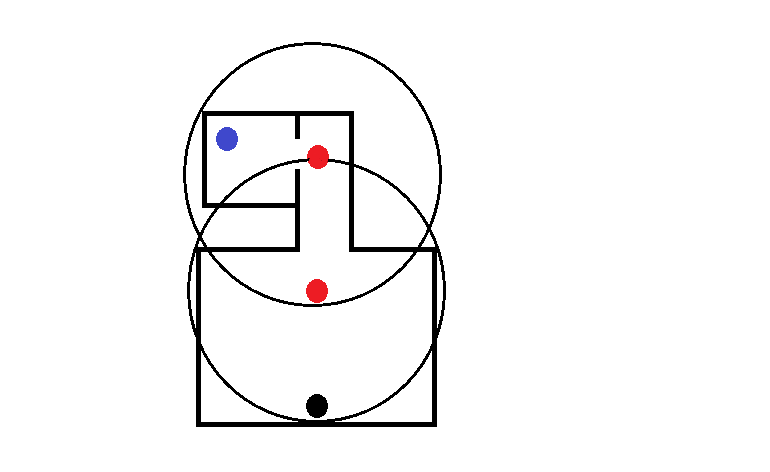
\includegraphics[width = 0.8\textwidth]{../../figures/comm_example_room.png} 
\caption{An example of the communication link needed for rooms}
\label{comm_example_room}
\end{figure}


The theory of what could be  implemented uses a defined maximum communication range for the robots and a grouping strategy which specifies that each scout robot need to stay in contact which at least 1 comm robot while the comm robots always need at least 1 other comm robot inside their communication range. If implemented correctly the comm robots would on this way create a communication link back to the lead robot/starting location which the scout robots can use to transfer all new information back.\\

\begin{figure}[h]
\centering
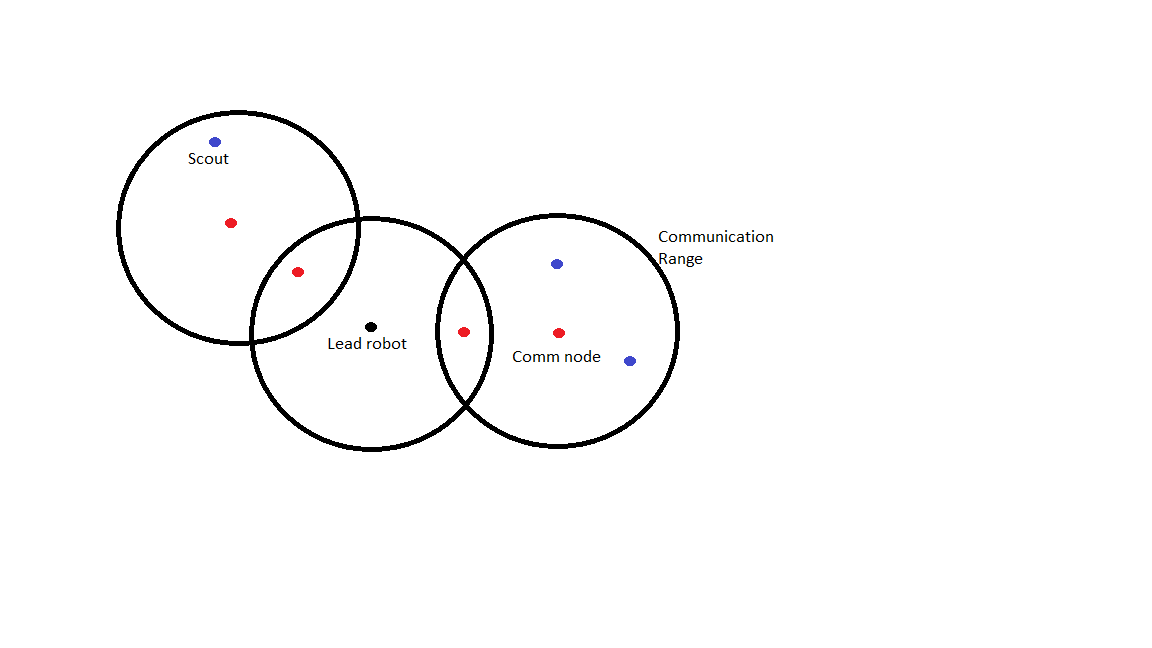
\includegraphics[width = 0.8\textwidth]{../../figures/comm_example.png} 
\caption{An example of the communication link}
\label{comm_link_example}
\end{figure}

Figure \ref{comm_link_example} shows one possible example of the communication link, where the lead robot or in some cases a stationary uplink point is in the center and the communication robots(in red) placed in such positions that their comm range overlaps the comm range of other robots and the lead robot. \\
This configuration allows the scouts(in blue) to move and explore anything inside the communication range of the different comm robots. When the robots at the right side of the figure would now try to move outside the comm range one of them would have to change their behaviour pattern to "communication mode" at the outer range of the other comm nodes range while the last remaining scout continuous exploring in this direction. \\
This example shows that it is important to have a swarm of a suitable size for an environment to be able to cover at much area with the robots at hand and for cases in which this is not possible to be able to move the whole swarm in one unified direction to explore unmapped locations. This is however only doable when there is a lead robot since a stationary comm/uplink point is by definition, stationary.\\

\subsection{Swarm deployment}
The deployment strategy is an important part of a  project like this  as it defines how effective the swarm will cover the target area which will define how long it will take to scan and map the whole area. Another important aspect is how many robots can the swarm hold and effectively deploy using the current deployment strategy. \\ 
One research paper which was found proposed an solution of a communication network where the comm nodes keep track of the robots positions and guide them in directions which have not been explored in the last time period\cite{Batalin2003Coverage}. The paper uses a solution which is based on small comm nodes deployed by the robot, to make the solution fitting for this project it would be necessary to define some of my E-pucks as communication nodes which remain on a fast position and guide the "scout" E-pucks based on area which have been least visited by the other robots.\\ 
This is certainly an possible solution however it could be considered a waste of robots in an small environment. Since an simulator is used there is no communication range problem, but as the indentions are to make it as close to a possible real world application as possible this must still be considered. 
That is why an maximum communication range for the robots needs to be implemented however more about that can be found in section \ref{communication}.\\[3ex]

Another paper proposed an solution which is based on an Nearest-Neighbour algorithm, meaning every robot must have always a minimum of "N" other robots inside its communication range\cite{Poduri2004Constrained}. In this solution to robots would emit signals to other robots which would manoeuvre the robots away from each other until only "N" robots remain inside the robots communication range. \\
This solution would cover a large area with the swarm fairly fast and also be adaptable for a swarm of any size, however a solution of moving the whole swarm in on direction would be needed in order to cover the whole target area, assuming the robot swarm is not big enough to cover it once completely deployed.
This would therefore need both a lead robot which decides the movement of the swarm and communication robots which would always have at least 1 link to another comm robot in order to have a communication line back to the lead robot. \\
These are 2 deployment strategies ideas which were found during the background reading.  \\[3ex]

Another approach could be to use a similar approach as is taken during the project so far, using an rectangular movement pattern for each robot. This could be a reasonable approach when the approximate size of the environment is known\cite{Mei2006Deployment}.

\begin{figure}[h]
\centering
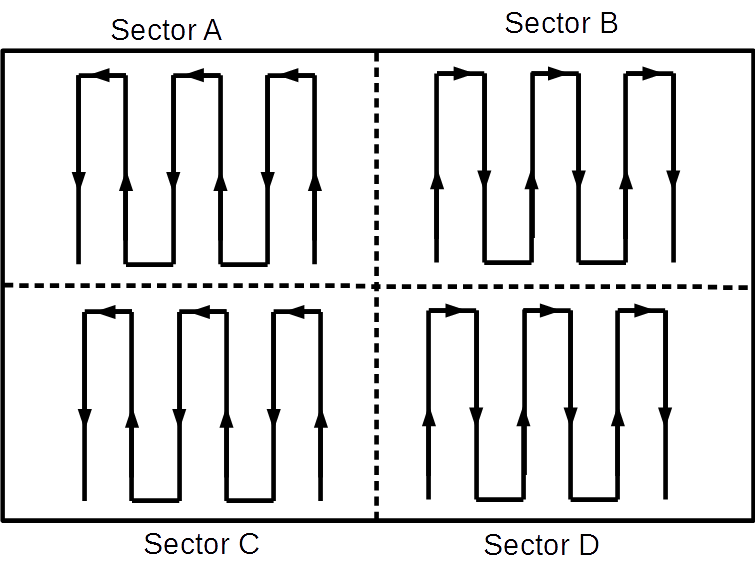
\includegraphics[width = 0.8\textwidth]{../../figures/deployment_sector_pattern} 
\caption{Sector based deployment pattern}
\label{deployment_sector_pattern}
\end{figure}

Figure \ref{deployment_sector_pattern} shows how a deployment pattern similar to the one implemented inside the project now. 
The altered deployment pattern would be based on splitting up the environment into scan sectors. Were each robot, in this case 4, would get an sector allocated which it will then proceed to scan. This however would require at least an reasonable estimate about  the environment size, in order to specify into how many sectors the environment would be split up. \\[3ex]

However this approach would require a swarm fitting to the environment size, where of the previous discussed deployment methods are able to traverse large environment even with smaller swarms, however for this circumstances an advanced movement pattern which is able to move the whole swarm in one direction would be needed.\\
However the sector moving pattern would work best, maybe even only, in square environment where as it most likely would fail in more advanced environments.

\section{Autonomous Swarm behaviour}
The previous sections describes different deployment strategies and addresses the communication problem, however one feature which could be implemented is intelligent robot behaviour in form of finding unexplored areas automatically. \\
This feature would depend heavily on that functioning deployment and communication algorithms are in place. The aspect of this algorithm would be to detect an unexplored area by checking the already created map. The idea for this is to ,as an example, scan an room which is connected to another room through a doorway. This would requite the map to be good enough and the doorway to be distinctive enough from the rest of the environment to be able to picked up. \\

\begin{figure}[h]
\centering
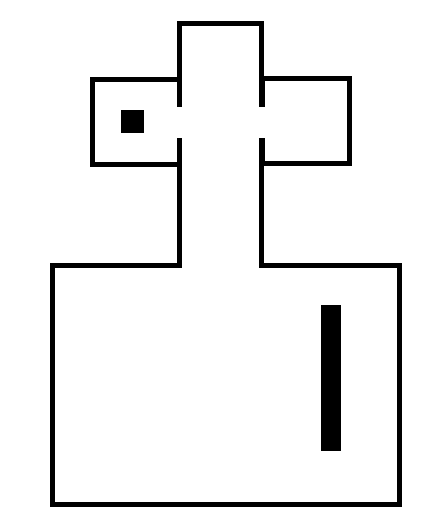
\includegraphics[width = 0.8\textwidth]{../../figures/environment_example} 
\caption{Example of an advanced environment}
\label{environment_example}
\end{figure}

Figure \ref{environment_example} shows a example of an advanced environment, for which such a autonomous behaviour would be needed in order to first, move the robots into the corridor and after that into the adjacent rooms. This is assuming the swarm starts in the large area at the bottom. \\



